%-- Add sections and your outline will be created automatically --%
\subsection{Backward facing step}

\begin{frame}
    \frametitle{Backward facing step (2D and 3D)}
\begin{itemize}
\item Classic CFD test case
\item Experimental and numerical data available for comparison
\item Test of numerical methods or turbulence models
\item Serial/parallel run
\end{itemize}
\begin{figure}
\centering
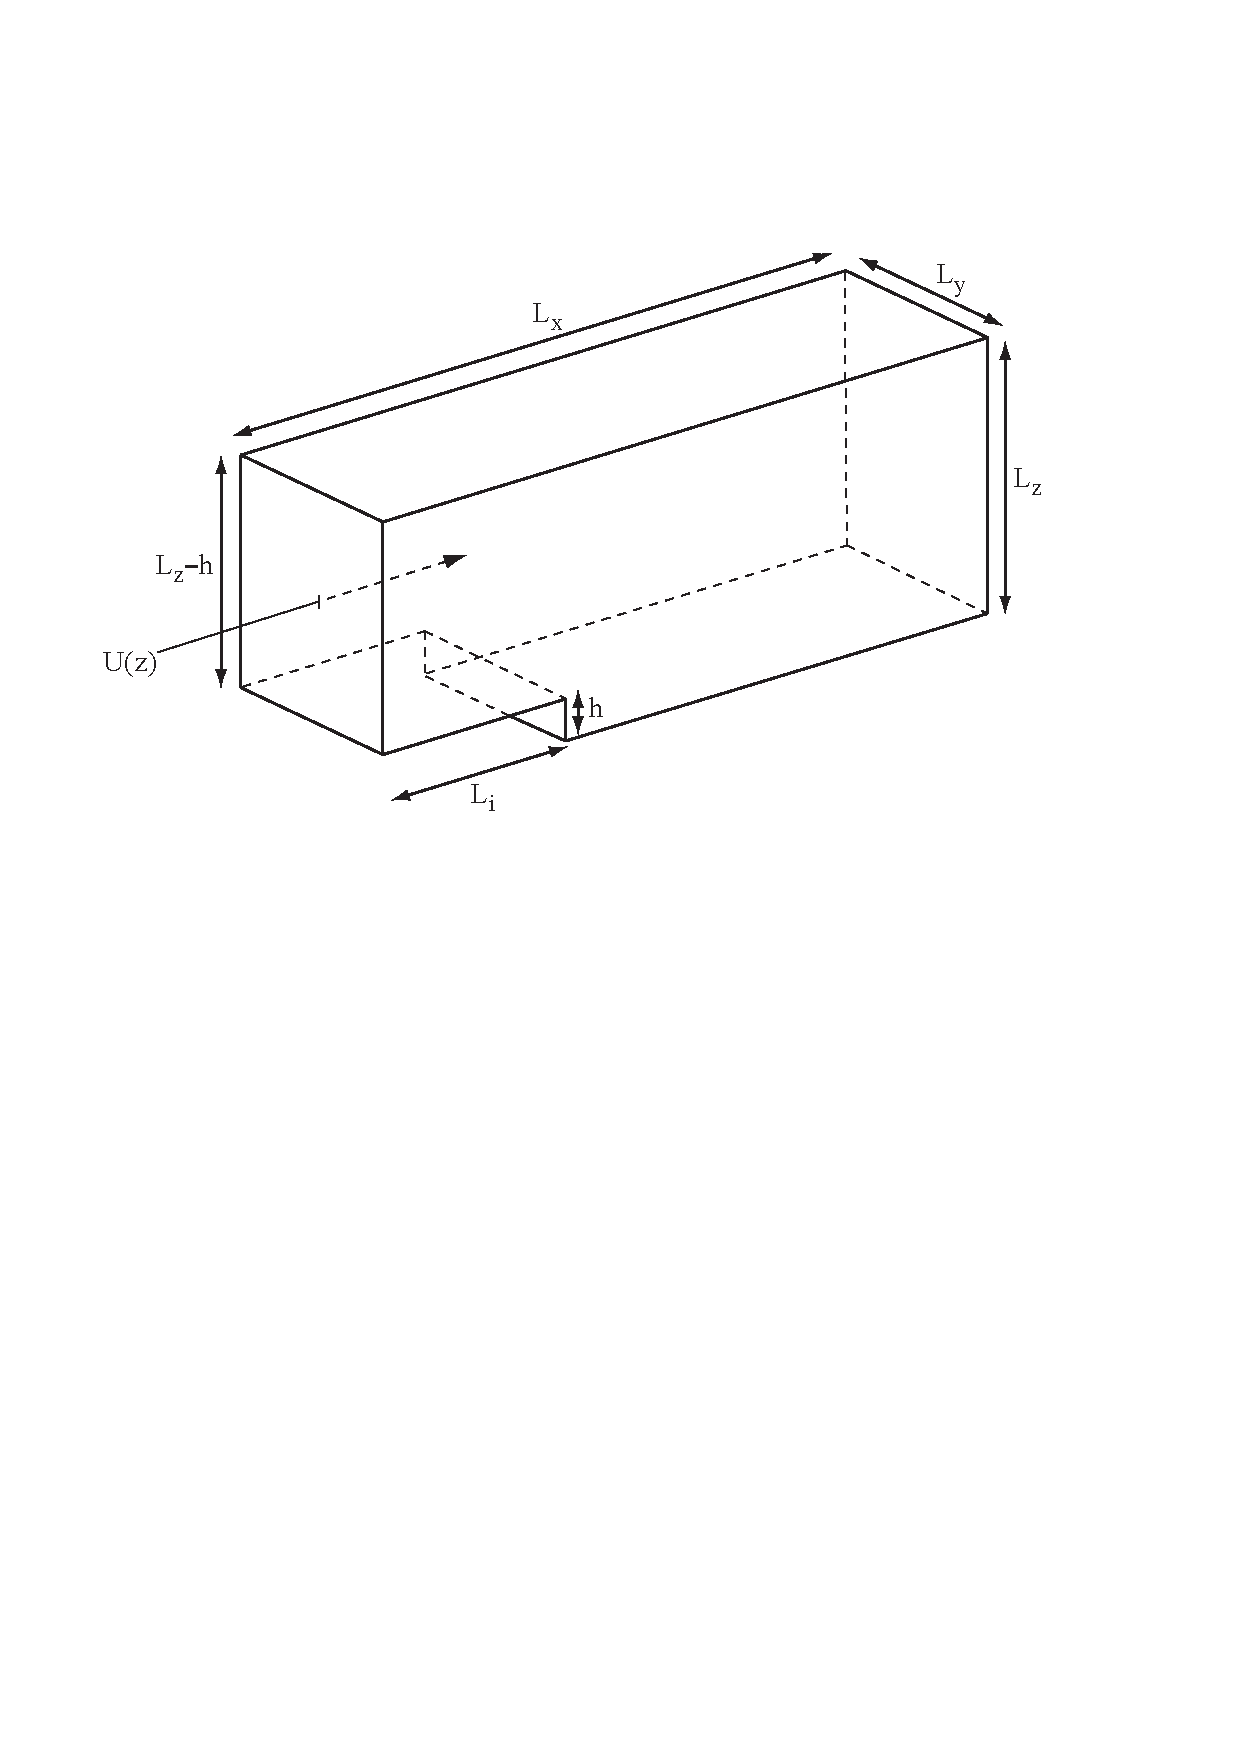
\includegraphics[width=0.5\textwidth]{./backward_facing_step/backward_facing_step_3d-schematic}
\caption{Geometry of 3D backward facing step}
\end{figure}
\end{frame}
%
\begin{frame}
    \frametitle{Backward facing step (2D and 3D)}
\begin{itemize}
\item Simulation run in serial.
\end{itemize}
\begin{figure}
\centering
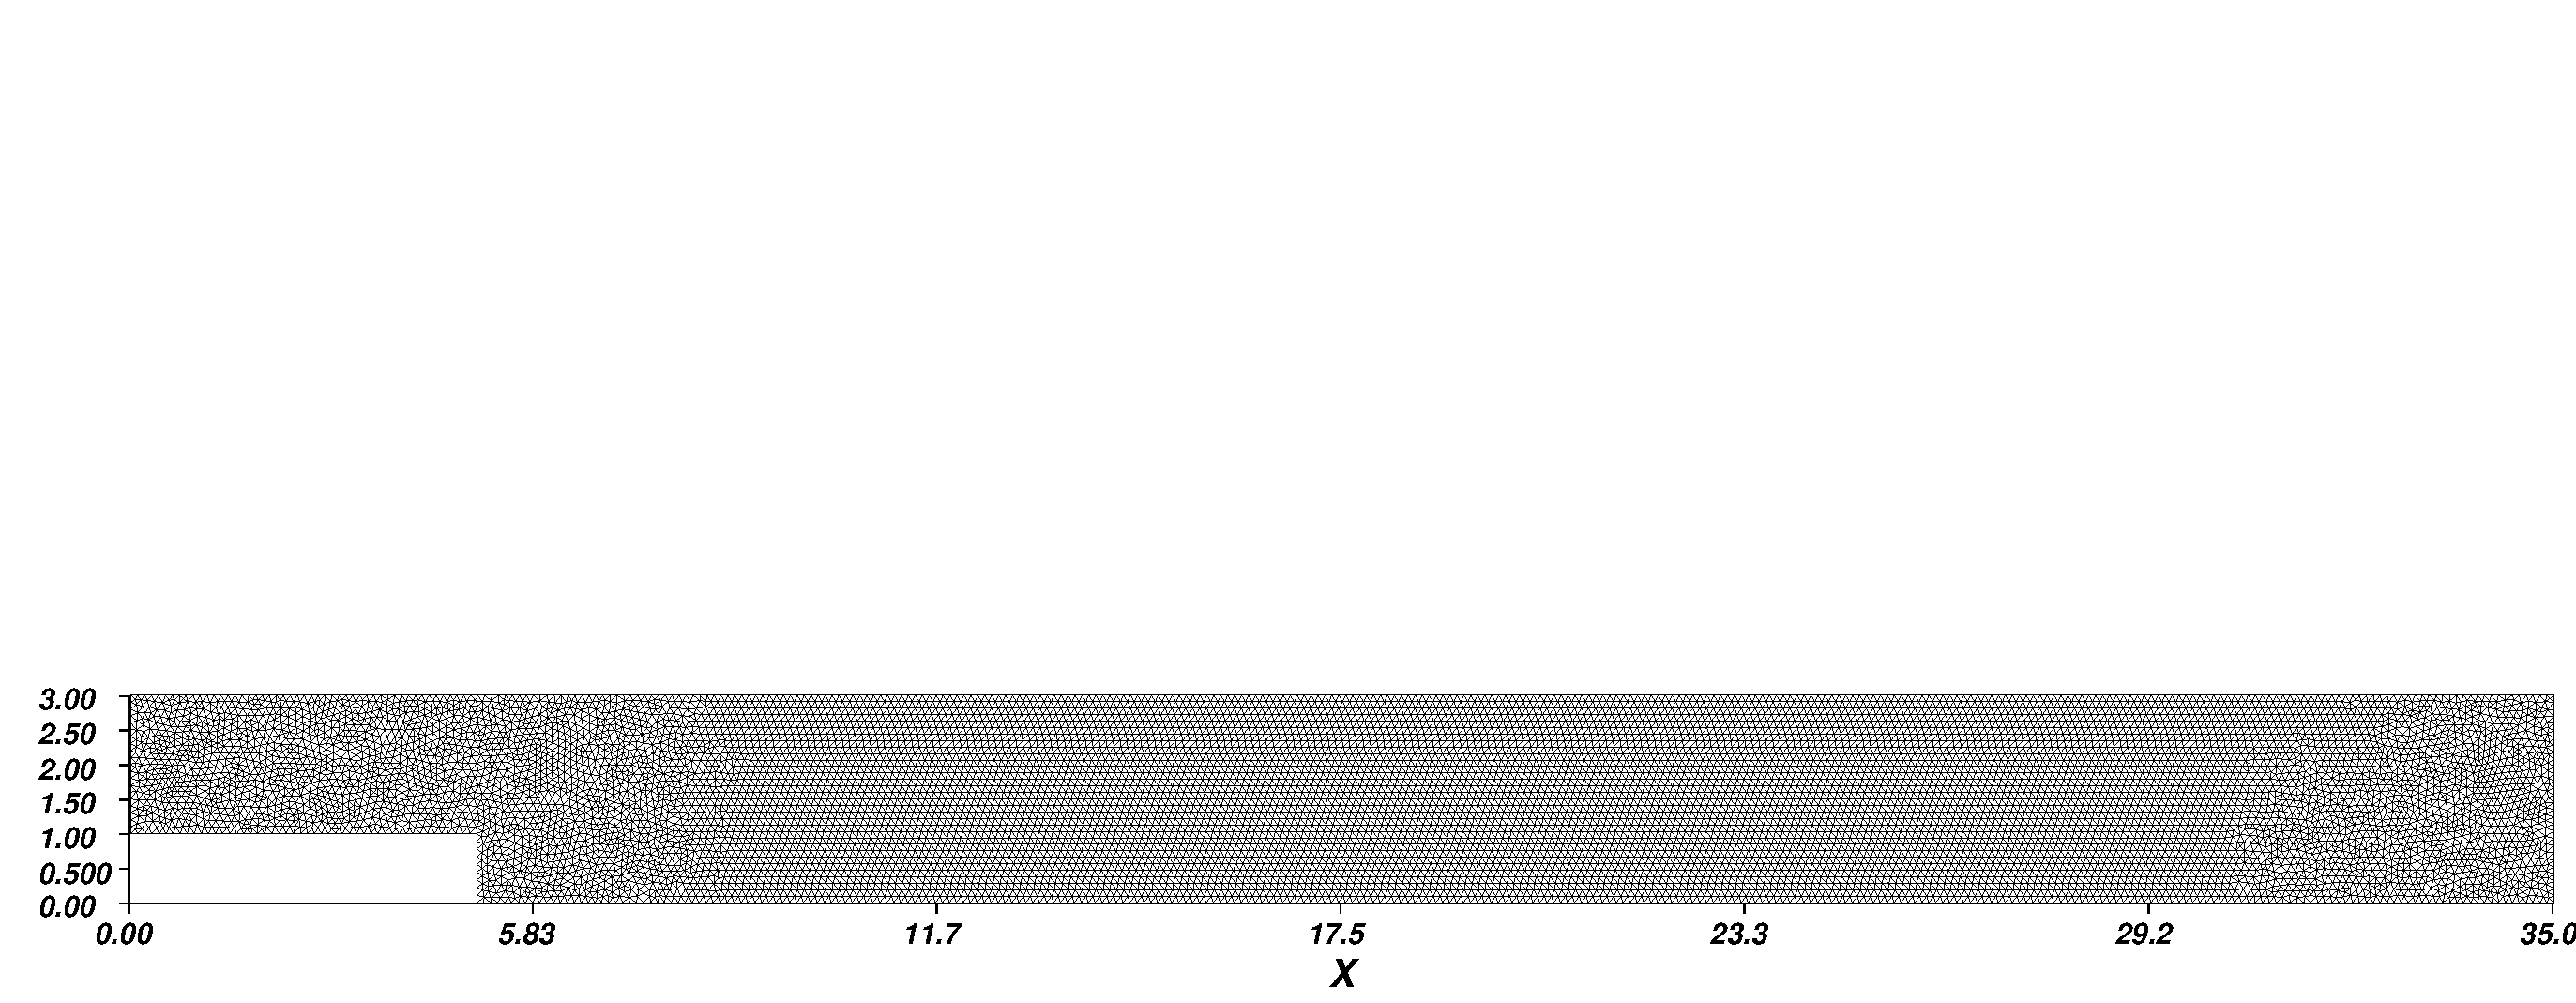
\includegraphics[width=1.0\textwidth]{./backward_facing_step/backward_facing_step_2d-mesh}
\caption{Geometry of 2D backward facing step showing the mesh.}
\end{figure}
\end{frame}
%
\begin{frame}
    \frametitle{Backward facing step, 2D results}
\begin{itemize}
\item Reattachment point estimation
\item Profile evolution in time/space
\end{itemize}
\begin{figure}
\centering
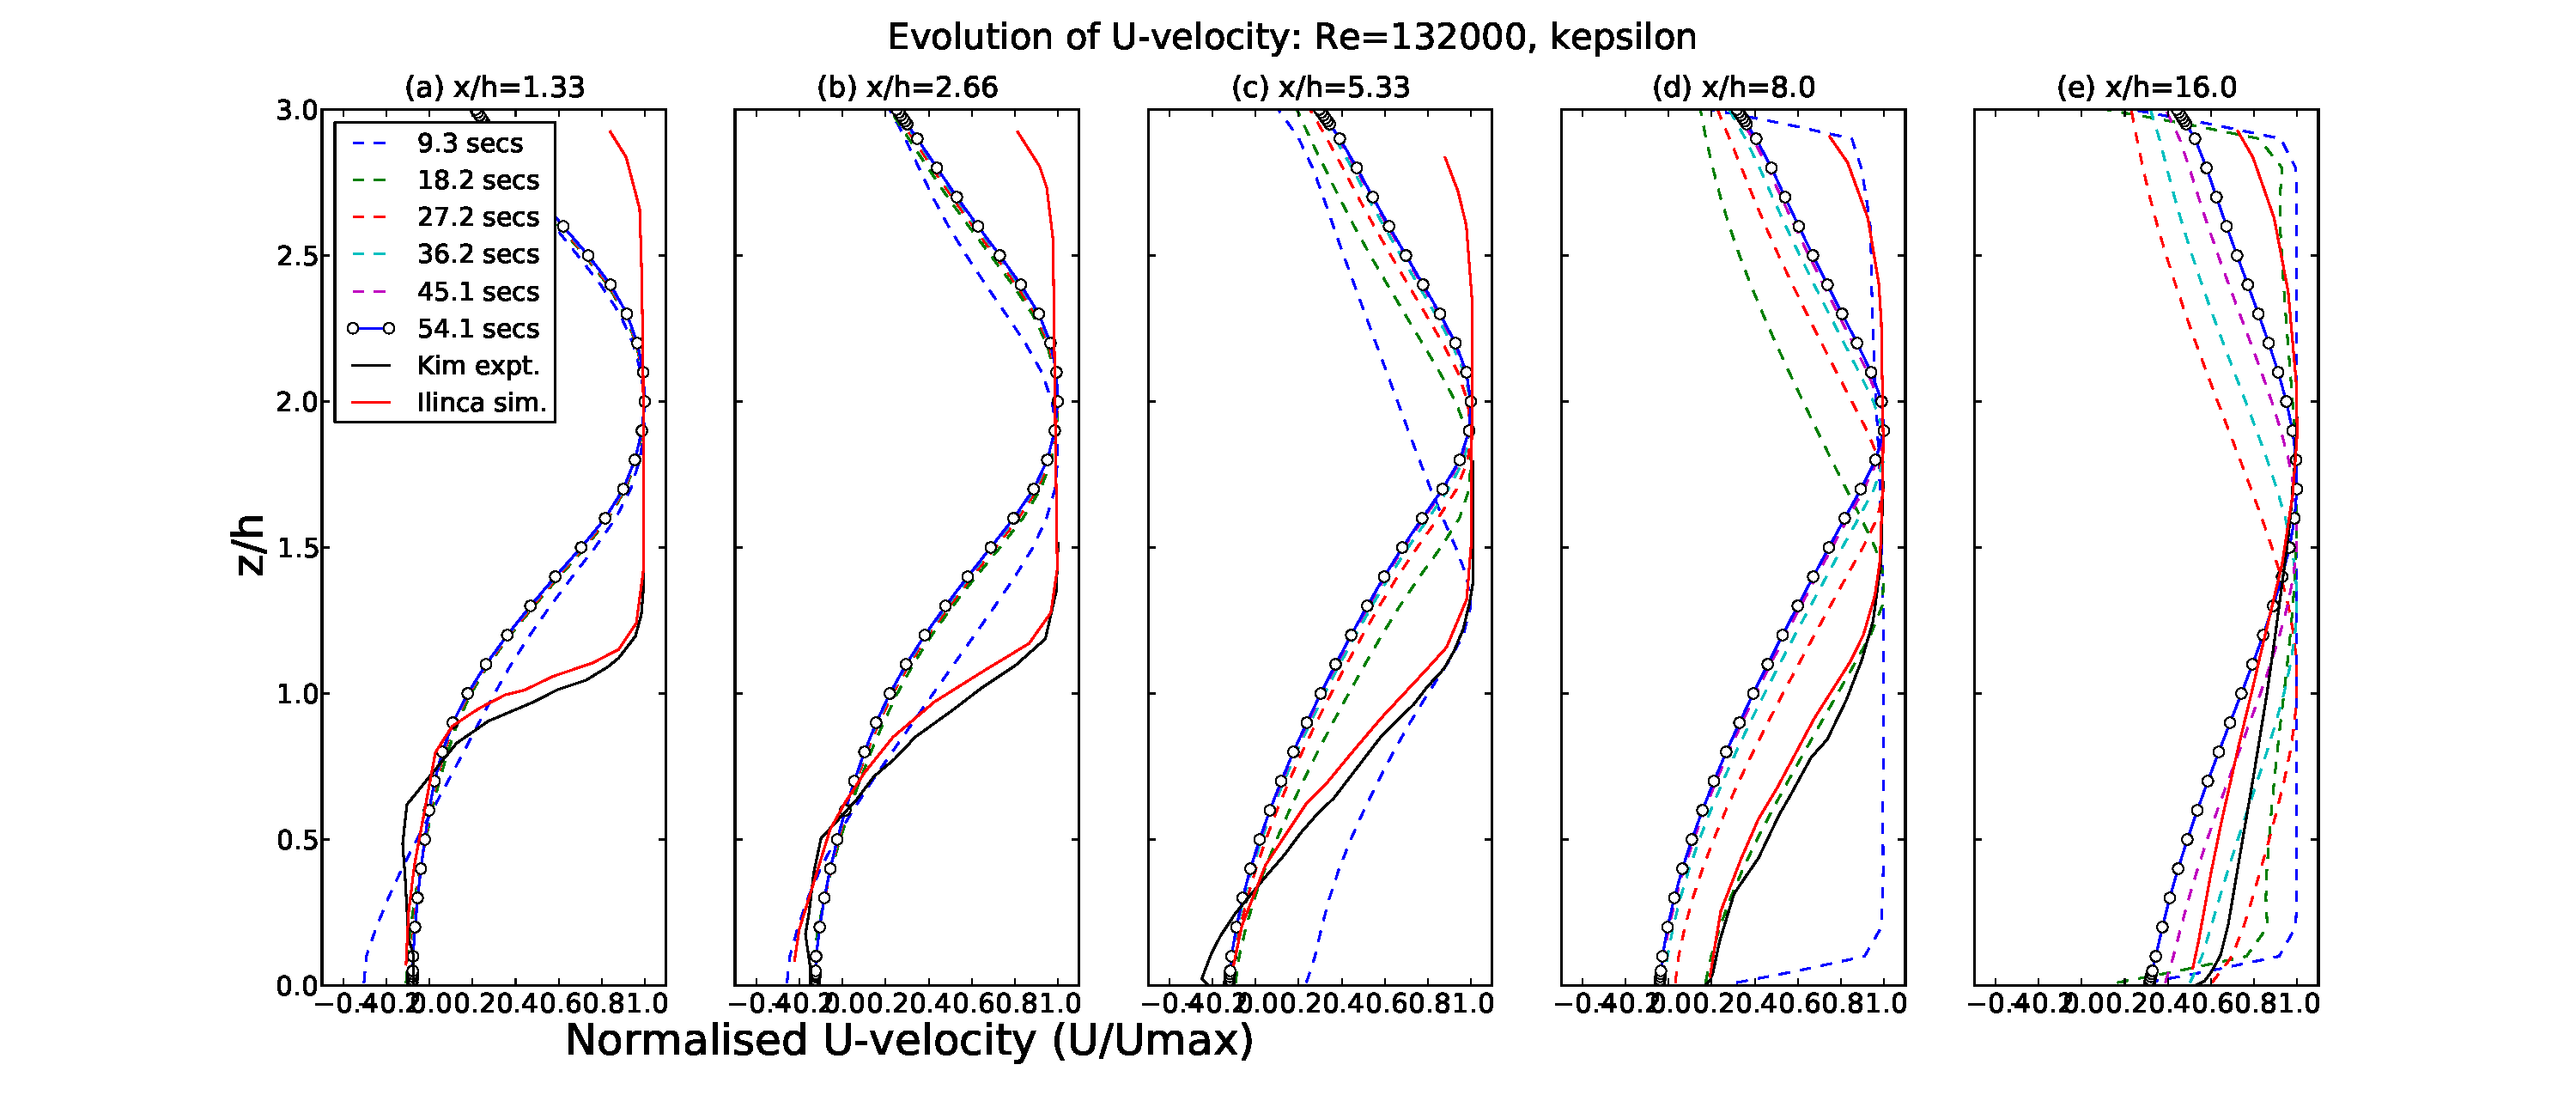
\includegraphics[width=0.7\textwidth]{./backward_facing_step/velocity_profiles_kim_kepsilon}
\caption{Streamwise velocity profiles at several points downstream of the step showing the converged solution and comparing to experimental and other numerical data.}
\end{figure}

\end{frame}
%
\begin{frame}
    \frametitle{Backward facing step, 3D results}
\begin{itemize}
\item Recirculation bubble and reattachment point
\end{itemize}

\begin{figure}
\centering
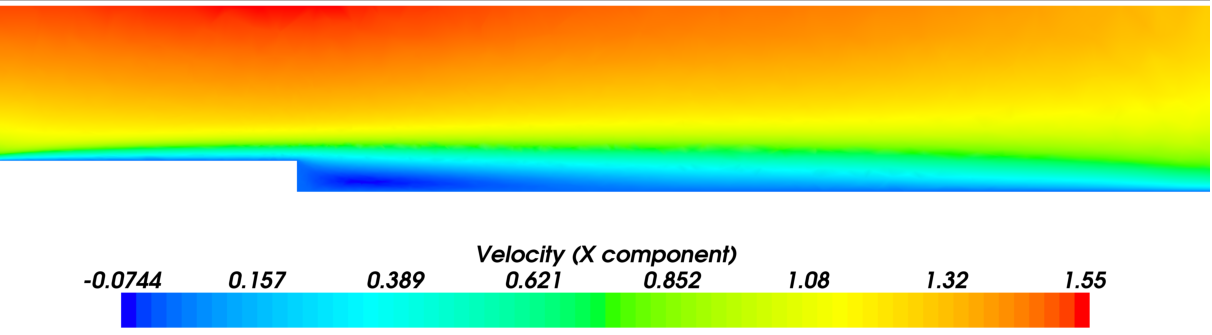
\includegraphics[width=0.8\textwidth]{./backward_facing_step/velo-magnitude-3d-50sec}
\caption{Velocity cut plane through centre of 3D geometry, time $=50\,$s.}
\end{figure}

\end{frame}
%
\begin{frame}
    \frametitle{Backward facing step, exercises}
\begin{itemize}
\item Increase the Reynolds number.
\item Add adaptivity options for both 2D and 3D.
\end{itemize}

\end{frame}
